\documentclass[14pt]{beamer}

% font
\usepackage{fontspec}
\setmainfont[Ligatures=TeX]{IPAPGothic}
\usepackage{xeCJK}
\setCJKmainfont{IPAPGothic}
\newfontfamily{\liberation}{Liberation Sans}
\newfontfamily{\notosans}{Noto Sans}

% graphic
\usepackage{graphics}
\usepackage{graphicx}
\usepackage{color}
\usepackage{xcolor}
\usepackage{colortbl}
\definecolor{mygray}{rgb}{0.1, 0.1, 0.1}

% tikz
\usepackage{tikz}
\usetikzlibrary{automata}
\usetikzlibrary{arrows}
\usetikzlibrary{arrows.meta}
\usetikzlibrary{positioning}
\usetikzlibrary{intersections, calc}
\usetikzlibrary{decorations}
\usetikzlibrary{decorations.markings}
\usetikzlibrary{decorations.pathreplacing,angles,quotes}
\usetikzlibrary{fit}
\usetikzlibrary{math}
\usetikzlibrary{shapes}
\usepackage{pgfplots}
\usepackage{bchart}

% href
\usepackage{hyperref}
\hypersetup{
	colorlinks=true,
	linkcolor=cyan,
	filecolor=cyan,
	urlcolor=cyan,
	pdfnewwindow=true}

% beamer
\usepackage{bxdpx-beamer}
\usetheme{Boadilla}
\setbeamertemplate{navigation symbols}{}
\setbeamercovered{transparent}
\setbeamertemplate{frametitle}{%
	\vspace{0.1em}
	\usebeamerfont{frametitle}\insertframetitle%
	\par
	\rule[0.5\baselineskip]{0.9\paperwidth}{0.4pt}%
	\vspace{-0.5em}}
\setbeamertemplate{footline}{
	\hfill
	\usebeamercolor[fg]{page number in head/foot}
	\usebeamerfont{page number in head/foot}
	{\small \insertframenumber}
	\kern1em\vskip5pt
}
\setbeamercolor{footline}{fg=black,bg=black}

% itemize
\usepackage{enumitem}
\setitemize{itemsep=0.2em}
\setlength\leftmargini{20pt}
\setlength\leftmarginii{20pt}
\setlength\leftmarginiii{20pt}
\setlength\leftmarginiv{20pt}
\setlist[itemize,1]{label=$\color{blue}\bullet$}
\setlist[itemize,2]{label=$\color{orange}\triangleright$}
\setlist[itemize,3]{label=$\color{gray}\bullet$}
\setlist[itemize,4]{label=$\color{red}\triangleright$}
\setlist[itemize,5]{label=$\color{gray}\bullet$}
\setlist[itemize,6]{label=$\color{red}\triangleright$}
\setlist[itemize,7]{label=$\color{yellow}\bullet$}
\setlist[itemize,8]{label=$\color{pink}\triangleright$}
\setlist[itemize,9]{label=$\color{black}\bullet$}

% math
\usepackage{amsmath,amssymb,amsthm}
\usepackage{bm}

% other
\usepackage{caption}
\usepackage{cancel}
\usepackage{epigraph}
\usepackage{fancybox}
\usepackage{here}
\usepackage{makecell}
\usepackage{setspace}
\usepackage{scrextend}
\usepackage{svg}
\usepackage{ulem}
\usepackage{multirow}

\begin{document}

\begin{frame}
	\begin{center}
		{\huge \color{cyan} そうぇり もぷもぷ}
	\end{center}
\end{frame}


\begin{frame}
	\frametitle{soweli Mopumopu}
	
	\begin{itemize}
		\item Twitter上のトキポナボット
			\begin{itemize}
				\item \href{https://twitter.com/soweli_mopumopu}{@soweli\_mopumopu}
			\end{itemize}
	\end{itemize}
	
	\begin{figure}[H]
		\centering
		
\includegraphics[width=10cm]{mopumopu.png}
	\end{figure}
\end{frame}

\begin{frame}
	\frametitle{soweli Mopumopu}
	
	\begin{itemize}
		\item 15分おきに何か言葉を発します
		\item 会話もできます たのしいね
	\end{itemize}
	
	\begin{figure}[H]
		\centering
		\begin{minipage}{0.45\linewidth}
			
\includegraphics[height=2.7cm]{mopu1.png}
		\end{minipage}
		\begin{minipage}{0.45\linewidth}
			
\includegraphics[height=2.7cm]{mopu2.png}
		\end{minipage}
	\end{figure}
\end{frame}

\begin{frame}
	\frametitle{なんの話をするの}

	\begin{itemize}
		\item soweli Mopumopuはどうやって動いてるのか?
			\begin{itemize}
				\item 実はすこし高度なことをしている
			\end{itemize}
		\item もぷもぷの技術について説明します
	\end{itemize}
\end{frame}

\begin{frame}
	\frametitle{トキポナとは}

	\begin{itemize}
		\item みんなが知ってるミニマル言語
			\begin{itemize}
				\item 語彙数: 120語
				\item 習得がかんたん たのしい!
				\item できる人が割と多い たのしい!
			\end{itemize}
		\item 知らない人のために
			\begin{itemize}
				\item \href{https://twitter.com/notolytos/status/1409484535151042568}{\small 初級トキポナ文法簡介}
				\item \href{https://www.youtube.com/watch?v=9C0YqTs4vB8}{\small 2分40秒で世界一簡単な言語を紹介して伝授する}
				\item \href{https://www.youtube.com/watch?v=wIFJfAhiPlE}{\small トキポナレッスン1「トキポナってなに」}
				\item \href{https://en.wikibooks.org/wiki/Updated\_jan\_Pije\%27s\_lessons}{\small jan Pije's lessons} 
					{\scriptsize (\href{https://github.com/stefichjo/toki-pona/blob/master/pije.md}{注})}
				\item \href{https://www.youtube.com/watch?v=2jRtYBaZGgQ}{\small 【日本語訳】toki pona li toki pona - トキポナソング}
			\end{itemize}
	\end{itemize}
\end{frame}

\begin{frame}
	\frametitle{トキポナをモデル化する}

	\begin{itemize}
		\item トキポナをコンピュータで扱いたい!
			\begin{itemize}
				\item コンピュータには言語がわからぬ...
			\end{itemize}
		\item ``文''を数理モデル化しよう!
			\begin{itemize}
				\item 確率的言語というのを考えます
			\end{itemize}
	\end{itemize}
\end{frame}

\begin{frame}
	\frametitle{確率的言語}

	\begin{itemize}
		\item 「その文が起きる確率」というのを考える
			\begin{itemize}
				\item 文の確率$P(\text{文})$を考える
				\item $P(\text{toki pona li toki pona!})$とか
			\end{itemize}
		\item なにがうれしいの?
	\end{itemize}
\end{frame}

\begin{frame}
	\frametitle{確率的言語}

	\begin{itemize}
		\item 次の2つの文$A, B$はどちらが``良い''文だろうか?
			\begin{itemize}
				\item 文$A$: toki pona li toki pona.
				\item 文$B$: a akesi ala alasa ale.
					\begin{itemize}
						\item 明らかに$A$のほうがよい
						\item $P(A) > P(B)$となるはず
					\end{itemize}
				\item 確率的言語は文法を扱えるかも?
			\end{itemize}
	\end{itemize}
\end{frame}

\begin{frame}
	\frametitle{確率的言語}

	\begin{itemize}
		\item 次の2つの文$A, B$はどちらが``良い''文だろうか?
			\begin{itemize}
				\item 文$A$: ma tomo Tokijo li lon ma Nijon.
				\item 文$B$: ma tomo Lanten li lon ma Tosi.
					\begin{itemize}
						\item $A$は正しいが,$B$は間違い
						\item $P(A) > P(B)$となるはず
					\end{itemize}
				\item 確率的言語は意味や常識を扱えるかも?
			\end{itemize}
	\end{itemize}
\end{frame}

\begin{frame}
	\frametitle{確率的言語}

	\begin{itemize}
		\item 確率で言語を近似することができれば,文法や意味を捉えたモデルを作成できるのでは?
			\begin{itemize}
				\item ``良い文''・``悪い文''を定性的に評価できる
					\begin{itemize}
						\item チャットボットも作れる
					\end{itemize}
				\item もっと広く言語処理の様々な場面で使われている
					\begin{itemize}
						\item 機械翻訳などもこの考えを元に作られている
					\end{itemize}
			\end{itemize}
		\item 文の確率をどうやって計算するの?
	\end{itemize}
\end{frame}

\begin{frame}
	\frametitle{言語モデル}

	\begin{itemize}
		\item 文に確率を与えるモデルのこと
		\item つまり,
			\begin{itemize}
				\item 文$w_1^n = w_1 w_2 \cdots w_n$を入力して,
				\item $P(w_1^n)$を計算・出力する関数のようなもの
			\end{itemize}
		\item どのように計算する?
			\begin{itemize}
				\item そもそも入力の長さが文ごとに違うしつらい…
			\end{itemize}
	\end{itemize}
\end{frame}

\begin{frame}
	\frametitle{分解する}

	\begin{itemize}
		\item 確率論の乗法定理を用いて,$P(w_1^n)$を分解
	\end{itemize}
	\begin{align*}
		P(w_1^n)
			& = P(w_1, w_2, \cdots, w_n) \\
			& = P(w_1) P(w_2, w_3, \cdots, w_n | w_1) \\
			& = P(w_1) P(w_2 | w_1) P(w_3, w_4, \cdots, w_n | w_1, w_2) \\
			& = P(w_1) P(w_2 | w_1) P(w_3 | w_1^2) P(w_4^n | w_1^3) \\
			& = \prod_{i=1}^{n} P(w_i | w_1^{i-1})
	\end{align*}

	\begin{itemize}
		\item 1単語ずつ計算してかければ文の確率になる!
	\end{itemize}

\end{frame}

\begin{frame}
	\frametitle{$P(w_i | w_1^{i-1})$を計算する}

	\begin{itemize}
		\item $1$番目から$i-1$番目の単語がわかってて,$i$番目の単語が起こる確率
		\item $P(\text{li} | \text{toki pona}) > P(\text{wile} | \text{toki pona})$ 
		\item Mopumopuでは,ニューラルネットを用いている
			\begin{itemize}
				\item ニューラル言語モデルっていう
			\end{itemize}
	\end{itemize}
\end{frame}

\begin{frame}
	\frametitle{Transformerモデル}

	\begin{itemize}
		\item Mopumopuで採用したニューラルモデル
			\begin{itemize}
				\item 2017年にGoogleの人たちが考案した
					\begin{itemize}
						\item Google翻訳のなかみもこれ
					\end{itemize}
			\end{itemize}
		\item 次からのスライドで細かいことを説明します
			\begin{itemize}
				\item {\scriptsize 注: ここで説明するのは,
					一般によく言われている
					Transformer Encoder-Decoderモデルのことではなく,
					Transformer言語モデルのことです.}
			\end{itemize}
	\end{itemize}
\end{frame}

\begin{frame}
	\frametitle{Transformerモデル}

	\begin{itemize}
		\item Transformerモデルは次の部分からなっている
			\begin{itemize}
				\item 単語 Embedding 層
				\item 位置 Embedding 層
				\item Self-attention 層
				\item Feed-forward 層
			\end{itemize}
	\end{itemize}

\end{frame}

\begin{frame}
	\frametitle{単語 Embedding 層}

	\begin{itemize}
		\item 単語をベクトルに変換する
			\begin{itemize}
				\item Mopumopuでは1024次元
				\item 逆(ベクトル->単語)もできる
			\end{itemize}
	\end{itemize}

	\begin{figure}[H]
		\centering
		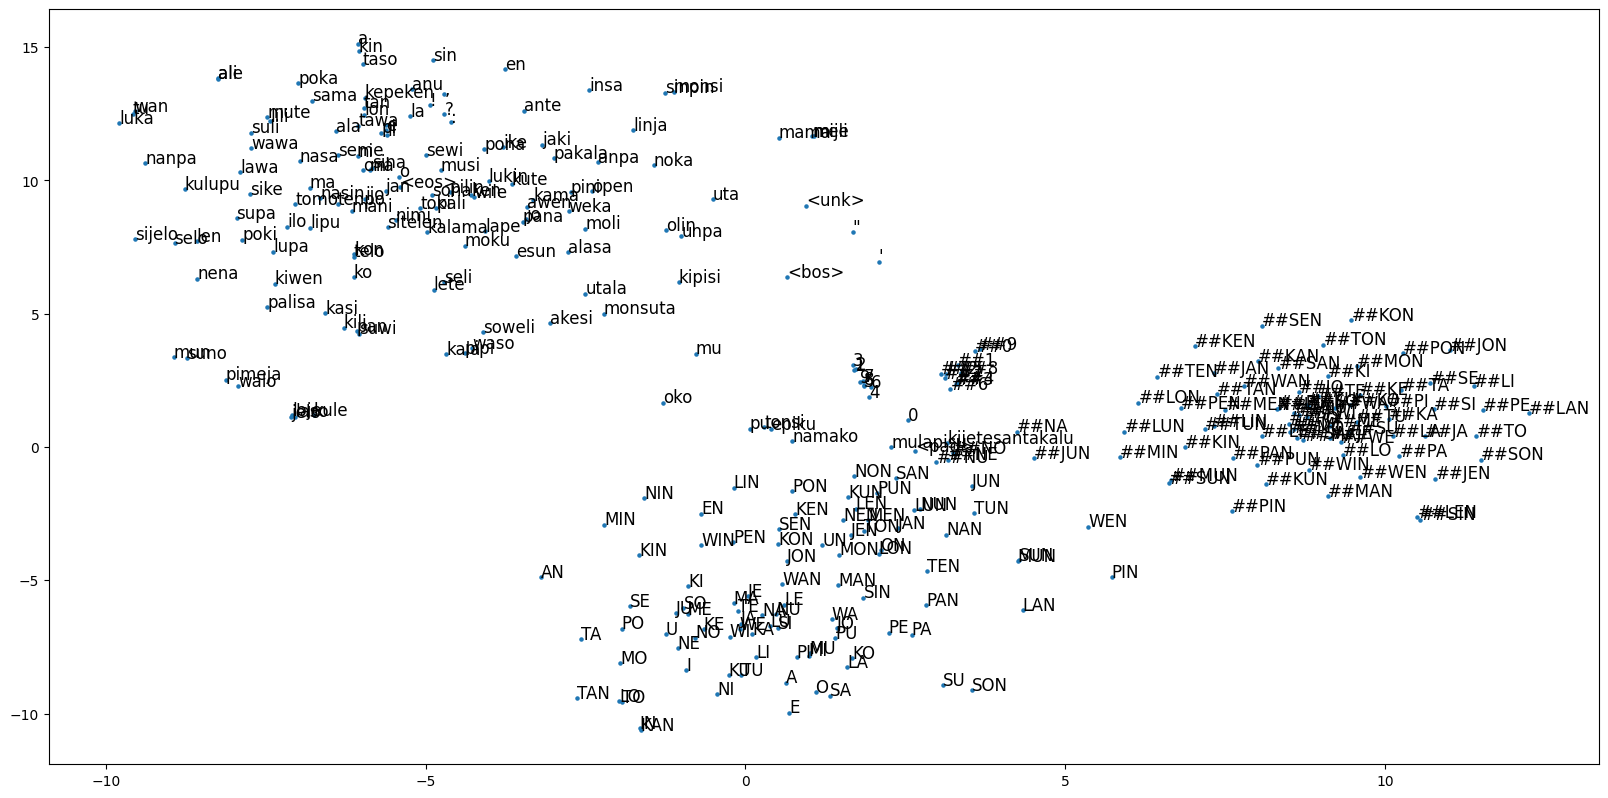
\includegraphics[width=10cm]{embed.png}
	\end{figure}
\end{frame}

\begin{frame}
	\frametitle{位置 Embedding 層 {\small (難しい)}}

	\begin{itemize}
		\item 位置(何番目の単語か)をベクトルで表す
			\begin{itemize}
				\item 三角関数の回転を利用している
				\item $t$番目の$i$次元が
					\[
						\bm{p}_t^{(i)}
						=
						\begin{cases}
							\sin \left( \omega_k t \right) & (i = 2k) \\
							\cos \left( \omega_k t \right) & (i = 2k + 1) \\
						\end{cases}
					\]
			\end{itemize}
	\end{itemize}
	\begin{figure}[H]
		\centering
		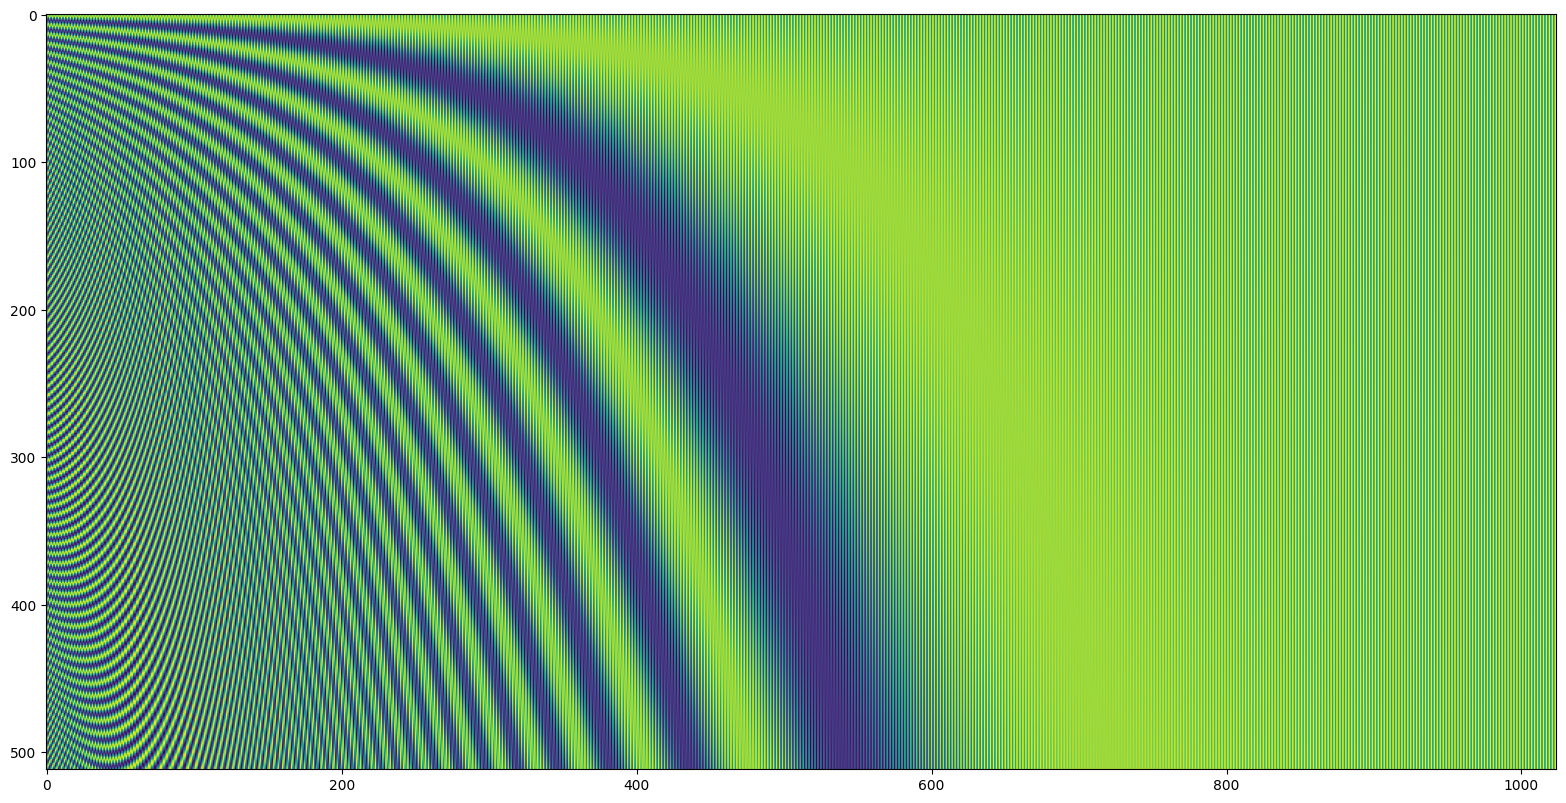
\includegraphics[width=7.5cm]{posenc.png}
	\end{figure}
\end{frame}

\begin{frame}
	\frametitle{Self-attention 層 {\small (難しい)}}

\end{frame}

\begin{frame}
	\frametitle{Feed-forward 層}

\end{frame}

\begin{frame}
	\frametitle{Transformerモデル}

	\begin{itemize}
		\item それをこんな感じで組み合わせると
	\end{itemize}

	\begin{figure}[H]
		\centering
		\begin{tikzpicture}[>=latex,font=\sffamily,scale=1.0,transform shape]
			\node[rectangle, text width = 3pt, text height = 70pt, draw = black] (a) at (0, 0) {};
			\node[rectangle, text width = 3pt, text height = 70pt, draw = black] (b) at (1, 0) {};
			\node[rectangle, text width = 3pt, text height = 70pt, draw = black] (c) at (2, 0) {};
			\node[rectangle, text width = 3pt, text height = 70pt, draw = black] (d) at (3, 0) {};
			\node[rectangle, text width = 3pt, text height = 70pt, draw = black] (e) at (4, 0) {};
			\node[rectangle, text width = 3pt, text height = 70pt, draw = black] (f) at (5, 0) {};
			\node[rectangle, text width = 3pt, text height = 70pt, draw = black] (g) at (6, 0) {};
			\node[rectangle, text width = 3pt, text height = 70pt, draw = black] (h) at (7, 0) {};
			\node[rectangle, text width = 3pt, text height = 70pt, draw = black] (i) at (8, 0) {};
			\draw[->] (a.east) -- (b.west);
			\draw[->] (b.east) -- (c.west);
			\draw[->] (c.east) -- (d.west);
			\draw[->] (d.east) -- (e.west);
			\draw[->] (e.east) -- (f.west);
			\draw[->] (f.east) -- (g.west);
			\draw[->] (g.east) -- (h.west);
			\draw[->] (h.east) -- (i.west);
			\node[rotate=90] at (0, 0) {\scriptsize 単語 Embedding 層};
			\node[rotate=90] at (1, 0) {\scriptsize 位置 Embedding 層};
			\node[rotate=90] at (2, 0) {\scriptsize Self-attention 層};
			\node[rotate=90] at (3, 0) {\scriptsize Feed-forward 層};
			\node[rotate=90] at (4, 0) {\scriptsize Self-attention 層};
			\node[rotate=90] at (5, 0) {\scriptsize Feed-forward 層};
			\node[rotate=90] at (6, 0) {\scriptsize Self-attention 層};
			\node[rotate=90] at (7, 0) {\scriptsize Feed-forward 層};
			\node[rotate=90] at (8, 0) {\scriptsize 単語 Embedding 層};
			\node[rotate=90] at (2.5, -1.7) {\scalebox{1}[3]{$\lbrace$}};
			\node[rotate=90] at (4.5, -1.7) {\scalebox{1}[3]{$\lbrace$}};
			\node[rotate=90] at (6.5, -1.7) {\scalebox{1}[3]{$\lbrace$}};
			\node (x) at (-1, 0) {\scriptsize 入力};
			\node (y) at (9, 0) {\scriptsize 出力};
			\draw[->] (x.east) -- (a.west);
			\draw[->] (i.east) -- (y.west);
		\end{tikzpicture}
	\end{figure}

	\begin{itemize}
		\item なんと言語モデルができる
	\end{itemize}

\end{frame}

\begin{frame}
	\frametitle{どのように学習するのか?}

	\begin{itemize}
		\item モデルの確率分布を言語の確率分布に近づける
			\begin{itemize}
				\item モデルと言語の相対エントロピーを小さくする
			\end{itemize}
	\end{itemize}
\end{frame}

\begin{frame}
	\frametitle{言語のエントロピー}
\end{frame}

\begin{frame}
	\frametitle{相対エントロピー}
\end{frame}

\begin{frame}
	\frametitle{クロスエントロピー}
\end{frame}

\begin{frame}
	\frametitle{確率的勾配降下法}

	\begin{itemize}
		\item クロスエントロピーを微分した方向の逆にモデルのパラメータを動かしていけば,
			小さくなっていくのでは?
			\begin{itemize}
				\item 「標高が低い方に進めば下山できるのでは?」
					\begin{itemize}
						\item[] \hspace{5em} {\scriptsize \color{lightgray} 遭難するのでやってはいけない}
					\end{itemize}
				\item 言語モデルが学習できる!
			\end{itemize}
		\item ほんとにこんなんで学習できるのか?
			\begin{itemize}
				\item 厳しいので工夫する
			\end{itemize}
	\end{itemize}
\end{frame}

\begin{frame}
	\frametitle{Adamアルゴリズム}

	\begin{itemize}
		\item a
	\end{itemize}

	(SDGの式に2つ修正点があって,1次の向きをおさえてるのと,2次の大きさをおさえてるのがあるんだって話をかけばいい)
\end{frame}

\begin{frame}
	\frametitle{自己回帰生成}
\end{frame}

\begin{frame}
	\frametitle{ランダムサンプリング}
\end{frame}

\begin{frame}
	\frametitle{ランダムサンプリングは厳しい}
\end{frame}

\begin{frame}
	\frametitle{top-pサンプリング}
\end{frame}

\begin{frame}
	\frametitle{PyTorch}
\end{frame}

\begin{frame}
	\frametitle{nymwa/ponapt}
\end{frame}

\begin{frame}
	\frametitle{実際に動かす}
\end{frame}

\begin{frame}
	\frametitle{言語モデルでチャットボットをつくる}

	\begin{itemize}
		\item ちょっと無理がある
		\item すこし怪しいことをしている
	\end{itemize}
\end{frame}

\begin{frame}
	\frametitle{Twitter APIを使う}
\end{frame}

\begin{frame}
	\frametitle{おわりに}
\end{frame}

\end{document}

